\documentclass[main.tex]{subfiles}
\begin{document}\newpage
\setdoublesep{0.35700 em}  % 'Bond Spacing'
\setatomsep{1.78500 em}    % 'Fixed Length'
\setbondoffset{0.18265 em} % 'Margin Width'
\newcommand{\bondwidth}{0.06642 em} % 'Line Width'
\setbondstyle{line width = \bondwidth}
\newgeometry{left=0.8in,right=0.8in, top=2.5cm,bottom=2.5cm}
\fancyhfoffset[E,O]{0pt}
\setlength{\columnsep}{30pt}
\begin{conclusion}
\end{conclusion}
%\setstretch{0.3}
\begin{multicols*}{2}\setcounter{numA}{1}  %\newcounter{numA}


{\raggedright\textsc{\textbf{The nature of light}}\par}

%%%%%%%PROBLEM
\begin{question}[ID=\the\value{numA}]\SetQuestionProperties{section-title=\nameref{sec:units}}
Calculate the following properties:
\begin{inparaenum}[(a)]
\item  The energy in joules of a radiation with frequency $2.0\times10^{18}$ Hz?
\item  The frequency of a radiation with energy $5.6\times10^{-20}$ J?
 \item   The energy in joules of a radiation with wavelength $653$ nm?
\end{inparaenum}
\end{question}
\begin{solution}
\begin{inparaenum}[(a)]
\item  $1.32\times10^{-15}$J
\item  $8.5\times10^{13}$Hz
\item   $3.03\times10^{-19}$J
\end{inparaenum}\hspace{0.1cm}\end{solution}\stepcounter{numA}
%%%%%%%%%%%%%%

%%%%%%%PROBLEM
\vspace{-0.5cm}
\begin{question}[ID=\the\value{numA}]\SetQuestionProperties{section-title=\nameref{sec:units}}
Calculate the following properties:
\begin{inparaenum}[(a)]
\item  The wavelength of a radiation with  energy $5.34\times10^{-16}$J?
\item   The wavelength of a radiation with  frequency of $3.4\times10^{14}$ Hz?  
 \end{inparaenum}
\end{question}
\begin{solution}
\begin{inparaenum}[(a)]
\item   $0.37$ nm
\item   $882$ nm    
\end{inparaenum}\hspace{0.1cm}\end{solution}\stepcounter{numA}
%%%%%%%%%%%%%%
%%%%%%%PROBLEM
\vspace{-0.5cm}\begin{question}[ID=\the\value{numA}]\SetQuestionProperties{section-title=\nameref{sec:units}}
Calculate the following properties:
\begin{inparaenum}[(a)]
\item   The color of a radiation with $\lambda$= 510nm.
\item    Indicate the color of a radiation with $\lambda$= 580nm.
 \end{inparaenum}
\end{question}
\begin{solution}
\begin{inparaenum}[(a)]
\item    Green
\item    Yellow
\end{inparaenum}\hspace{0.1cm}\end{solution}\stepcounter{numA}
%%%%%%%%%%%%%%


%%%%%%%PROBLEM
\vspace{-0.5cm}\begin{question}[ID=\the\value{numA}]\SetQuestionProperties{section-title=\nameref{sec:units}}
Classify the nature of a radiation
\begin{inparaenum}[(a)]
\item    A radiation with $\gamma$= $3.4\times 10^{8}$Hz
\item     A radiation with $\lambda$= $1\times 10^{-4}$nm
 \end{inparaenum}
\end{question}
\begin{solution}
\begin{inparaenum}[(a)]
\item     Microwaves
\item     Gamma
\end{inparaenum}\hspace{0.1cm}\end{solution}\stepcounter{numA}
%%%%%%%%%%%%%%
 
%%%%%%%PROBLEM
\vspace{-0.5cm}\begin{question}[ID=\the\value{numA}]\SetQuestionProperties{section-title=\nameref{sec:units}}
Sections of two electromagnetic waves A and B  are represented below. Rank them in order of (a) increasing frequency; (b) increasing energy;  (c) If wave B represents visible radiation, is wave A more likely to be IR or UV radiation?  
\begin{centering}
     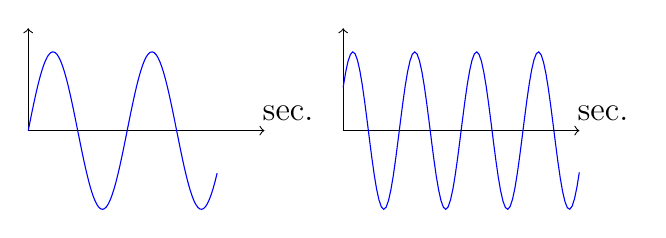
\begin{tikzpicture}[xscale=1,yscale=1]
      \begin{scope}[font=\itshape]
  \draw[->] (0,0) -- (0,1.3);
  \draw[->] (0,0)--(3,0) node[font=\large,black, above, pos = 1.1] {sec.};
  \draw[domain=0:2.4,samples=100,blue] plot(\x,{sin(\x r*5)});
   \draw[->] (4,0) -- (4,1.3);
  \draw[->] (4,0)--(7,0) node[font=\large,black, above , pos = 1.1] {sec.};
  \draw[domain=4:7.0,samples=100,blue] plot(\x,{sin(\x r*8)});
 \end{scope}
\end{tikzpicture}
     \end{centering}
\end{question}
\begin{solution}
\begin{inparaenum}[(a)]
\item     $\gamma_A$<$\gamma_B$
\item     $E_A$<$E_B$
\item IR
\end{inparaenum}
\hspace{0.1cm}\end{solution}\stepcounter{numA}
%%%%%%%%%%%%%%

%%%%%%%PROBLEM
\vspace{-0.5cm}\begin{question}[ID=\the\value{numA}]\SetQuestionProperties{section-title=\nameref{sec:units}}
Sections of two electromagnetic waves A and B  are represented below. Rank them in order of (a) increasing wavelength; (b) increasing energy;  (c) If wave B represents visible radiation, is wave A more likely to be IR or UV radiation?  
\begin{centering}
     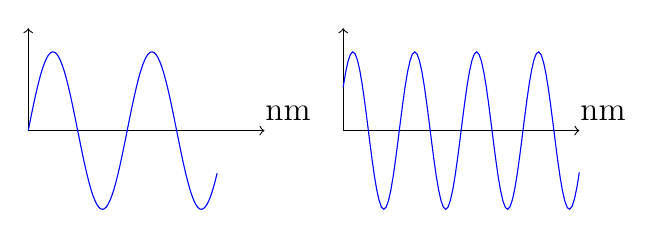
\begin{tikzpicture}[xscale=1,yscale=1]
      \begin{scope}[font=\itshape]
  \draw[->] (0,0) -- (0,1.3);
  \draw[->] (0,0)--(3,0) node[font=\large,black, above, pos = 1.1] {nm};
  \draw[domain=0:2.4,samples=100,blue] plot(\x,{sin(\x r*5)});
   \draw[->] (4,0) -- (4,1.3);
  \draw[->] (4,0)--(7,0) node[font=\large,black, above , pos = 1.1] {nm};
  \draw[domain=4:7.0,samples=100,blue] plot(\x,{sin(\x r*8)});
 \end{scope}
\end{tikzpicture}
     \end{centering}
\end{question}
\begin{solution}
\begin{inparaenum}[(a)]
\item     $\lambda_B$<$\lambda_A$
\item     $E_A$<$E_B$
\item UV
\end{inparaenum}
\hspace{0.1cm}\end{solution}\stepcounter{numA}
%%%%%%%%%%%%%%
 {\raggedright\textsc{\textbf{The atomic spectrum of hydrogen }}\par}

%%%%%%%PROBLEM
\vspace{-0.0cm}\begin{question}[ID=\the\value{numA}]\SetQuestionProperties{section-title=\nameref{sec:units}}
Which of these electron transitions correspond to absorption of energy and which to emission?
\begin{enumerate}[label=(\alph*)]\begin{multicols*}{2}
\item $\Delta E_{1\rightarrow 2}$  %absorption 
\item $\Delta E_{2\rightarrow 1}$	%Emission
\item $\Delta E_{3\rightarrow 1}$	%Emission
\item  $\Delta E_{3\rightarrow 5}$	%absorption
\item $\Delta E_{5\rightarrow 3}$	%Emission
\item $\Delta E_{1\rightarrow 3}$	%absorption
\end{multicols*}\end{enumerate}
\end{question}
\begin{solution}
\begin{inparaenum}[(a)]
\item  Absorption 
\item  Emission
\item  Emission
\item  Absorption
\item  Emission
\item  Absorption
\end{inparaenum}\hspace{0.1cm}\end{solution}\stepcounter{numA}
%%%%%%%%%%%%%%

 
%%%%%%%PROBLEM
\vspace{-0.5cm}\begin{question}[ID=\the\value{numA}]\SetQuestionProperties{section-title=\nameref{sec:units}}
Use the Bohr equation to:
 \begin{inparaenum}[(a)]
\item   find the energy of the photon emitted when an H atom undergoes a transition from $n=1$ to $n=4$.
\item   find the wavelength (in nm) of the photon emitted when an H atom undergoes a transition from $n=2$ to $n=4$.
\end{inparaenum}
 \end{question}
\begin{solution}
\begin{inparaenum}[(a)]
\item   $2.04\times10^{-18}$ J
\item $485$ nm
\end{inparaenum}\hspace{0.1cm}\end{solution}\stepcounter{numA}
%%%%%%%%%%%%%%

%%%%%%%PROBLEM
\vspace{-0.5cm}\begin{question}[ID=\the\value{numA}]\SetQuestionProperties{section-title=\nameref{sec:units}}
Use the Bohr equation to  find the frequency (in Hz) of the photon emitted when an H atom undergoes a transition from $n=1$ to $n=5$.
 \end{question}
\begin{solution}
$3.16\times10^{15}$ Hz
\hspace{0.1cm}\end{solution}\stepcounter{numA}
%%%%%%%%%%%%%%
%%%%%%%PROBLEM
\vspace{-0.5cm}\begin{question}[ID=\the\value{numA}]\SetQuestionProperties{section-title=\nameref{sec:units}}
An electron in the lowest energy level of H atom absorbs a photon of wavelength 96.97 nm. Indicate the final energy level of the electron moved.
 \end{question}
\begin{solution}
 $n=5$
\hspace{0.1cm}\end{solution}\stepcounter{numA}
%%%%%%%%%%%%%%


{\raggedright\textsc{\textbf{Quantum mechanics and electronic structure }}\par}

%%%%%%%PROBLEM
\vspace{-0.0cm}\begin{question}[ID=\the\value{numA}]\SetQuestionProperties{section-title=\nameref{sec:units}}
Indicate the number of orbitals that can have the following designations:
 \begin{inparaenum}[(a)]
\item    2s   %1 orbital
\item    3p 	%3 orbitals
\item 0p	%0 orbital	
\item $n=4$	%16 orbitals
\end{inparaenum}
 \end{question}
\begin{solution}
 \begin{inparaenum}[(a)]
\item     1 orbital
\item     3 orbitals
\item  0 orbital	
\item  16 orbitals    
\end{inparaenum}
\hspace{0.1cm}\end{solution}\stepcounter{numA}
%%%%%%%%%%%%%%
%%%%%%%PROBLEM
\vspace{-0.5cm}\begin{question}[ID=\the\value{numA}]\SetQuestionProperties{section-title=\nameref{sec:units}}
Indicate if the following combination of quantum numbers are allowed:\\
\begin{tabularx}{\columnwidth}{>{}m{.20\linewidth} *{4}{Y} }
  \toprule
\heading{$n$} & \heading{$\ell$}  &  \heading{$m_\ell$} & \heading{$m_s$} & \heading{Allowed?}   \\
    \midrule
  4	&	4	&	1	&	$+^1/_2$    \\
   2	&	1&		4	&	$+^1/_2$   \\
4		&2	&	-2	&	$-^1/_2$\\    
    \bottomrule
\end{tabularx}
 \end{question}
\begin{solution}
\begin{tabularx}{\columnwidth}{>{}m{.20\linewidth} *{4}{Y} }
  \toprule
\heading{$n$} & \heading{$\ell$}  &  \heading{$m_\ell$} & \heading{$m_s$} & \heading{Allowed?}   \\
    \midrule
  4	&	4	&	1	&	$+^1/_2$ & no   \\
   2	&	1&		4	&	$+^1/_2$ & no  \\
4		&2	&	-2	&	$-^1/_2$&yes\\    
    \bottomrule
\end{tabularx}
\hspace{0.1cm}\end{solution}\stepcounter{numA}
%%%%%%%%%%%%%%

%%%%%%%PROBLEM
\vspace{-0.5cm}\begin{question}[ID=\the\value{numA}]\SetQuestionProperties{section-title=\nameref{sec:units}}
For each of the following sublevels, give the $n$ and $\ell$ values and the number of orbitals:  \begin{inparaenum}[(a)]
\item   6s 	  %($n=6;l=0$)
\item   4d 	  %($n=4;l=2$)
\item  2p	  %($n=2;l=1$) 
\end{inparaenum}
 \end{question}
\begin{solution}
 \begin{inparaenum}[(a)]
\item   6s 	  	($n=6;\ell=0$)
\item   4d 	  	($n=4;\ell=2$)
\item  2p	  	($n=2;\ell=1$)  
\end{inparaenum}
\hspace{0.1cm}\end{solution}\stepcounter{numA}
%%%%%%%%%%%%%%
%%%%%%%PROBLEM
\vspace{-0.5cm}\begin{question}[ID=\the\value{numA}]\SetQuestionProperties{section-title=\nameref{sec:units}}
What is the element with the electron configuration
\begin{inparaenum}[(a)]
\item   $1s^2 2s^2 2p^6 3s^2 3p^5$ 	  %(Cl)
\item   $1s^2 2s^2 2p^6 3s^2 3p^4$	  %(S)
\item $[Kr]5s^2 4d^8$  %(Pd)
\end{inparaenum}
 \end{question}
\begin{solution}
 \begin{inparaenum}[(a)]
\item   $1s^2 2s^2 2p^6 3s^2 3p^5$ 	   (Cl)
\item   $1s^2 2s^2 2p^6 3s^2 3p^4$	   (S)
\item $[Kr]5s^2 4d^8$   (Pd)
\end{inparaenum}
\hspace{0.1cm}\end{solution}\stepcounter{numA}
%%%%%%%%%%%%%%


{\raggedright\textsc{\textbf{Periodic Properties }}\par}

%%%%%%%PROBLEM
\vspace{-0.0cm}\begin{question}[ID=\the\value{numA}]\SetQuestionProperties{section-title=\nameref{sec:units}}
Among the elements, indicate the element with the largest atomic radius  
\begin{inparaenum}[(a)]
\item B
\item C
\item F
\item  Li
\item Na
\end{inparaenum}
 \end{question}
\begin{solution}
Na
\hspace{0.1cm}\end{solution}\stepcounter{numA}
%%%%%%%%%%%%%%

%%%%%%%PROBLEM
\vspace{-0.5cm}\begin{question}[ID=\the\value{numA}]\SetQuestionProperties{section-title=\nameref{sec:units}}
Among the elements, indicate the element with the largest ionization energy  
\begin{inparaenum}[(a)]
\item B
\item C
\item F
\item  Li
\item Na
\end{inparaenum}
 \end{question}
\begin{solution}
Na
\hspace{0.1cm}\end{solution}\stepcounter{numA}
%%%%%%%%%%%%%%
%%%%%%%PROBLEM
\vspace{-0.5cm}\begin{question}[ID=\the\value{numA}]\SetQuestionProperties{section-title=\nameref{sec:units}}
Among the elements, indicate the element with the largest electronegativity  
\begin{inparaenum}[(a)]
\item B
\item C
\item F
\item  Li
\end{inparaenum}
 \end{question}
\begin{solution}
F
\hspace{0.1cm}\end{solution}\stepcounter{numA}
%%%%%%%%%%%%%%
%%%%%%%PROBLEM
\vspace{-0.5cm}\begin{question}[ID=\the\value{numA}]\SetQuestionProperties{section-title=\nameref{sec:units}}
Among the elements, indicate the element with the largest metallic character  
\begin{inparaenum}[(a)]
\item B
\item C
\item F
\item  Li
\item Na
\end{inparaenum}
 \end{question}
\begin{solution}
Li
\hspace{0.1cm}\end{solution}\stepcounter{numA}
%%%%%%%%%%%%%%
 

 



\end{multicols*}
\newpage
\begin{answersenvironment}
\begin{minipage}[c]{1\textwidth}
\begin{localsize}{10}
{\Large \bf Answers}
\SetupExSheets{
  headings = inline-nr , % numbered and inline
  counter-format = qu) , % numbers 1) 2) ... 
}
%\printsolutions 
\printsolutions[byID={1,3,5,7,9,11,13,15,17}]
\end{localsize}
\end{minipage}\end{answersenvironment}

\end{document}











%

%


